% This is text associated with the open textbook "Open Electromagnetics"
% See immediately below for author, date
% This work is licensed under the Creative Commons Attribution-ShareAlike 4.0 International License. (CC BY-SA 4.0) 
% To view a copy of the license, visit http://creativecommons.org/licenses/by-sa/4.0/

%ORB TITLE Coaxial Line
%ORB AUTHOR 0        # S.W. Ellingson, Virginia Tech (ellingson@vt.edu)
%ORB DATE 20180802   # yyyymmdd
%ORB ABSTRACT

\label{m0143_Coaxial_Line} % <-- Must match name of this file and module directory name.  Don't mess with this!
\index{transmission line!coaxial|(}

Coaxial transmission lines consists of metallic inner and outer conductors separated by a spacer material as shown in Figure~\ref{m0143_fCoaxCrossSection}. 
The spacer material is typically a low-loss dielectric 
\index{dielectric (material)}
material having permeability approximately equal to that of free space ($\mu\approx\mu_0$) and permittivity $\epsilon_s$ that may range from very near $\epsilon_0$ (e.g., air-filled line) to 2--3 times $\epsilon_0$. 
The outer conductor is alternatively referred to as the ``shield,'' 
\index{shield}
since it typically provides a high degree of isolation from nearby objects and electromagnetic fields.
Coaxial line is single-ended\footnote{The references in ``Additional Reading'' at the end of this section may be helpful if you are not familiar with this concept.} in the sense that the conductor geometry is asymmetric and the shield is normally attached to ground at both ends.
These characteristics make coaxial line attractive for connecting single-ended circuits in widely-separated locations and for connecting antennas to receivers and transmitters.
%
\begin{figure}
\begin{center}
\pdftooltip{{  % note double braces
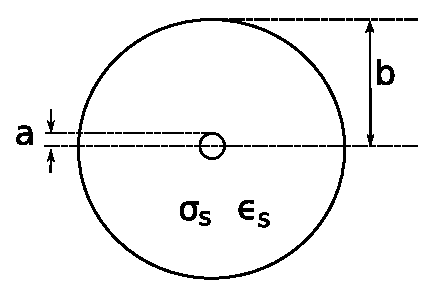
\includegraphics[width=2in]{modules/m0143_fCoaxCrossSection.eps}
}}{A small circle is concentric with a much larger circle. The radius of the small circle is called "a". The radius of the larger circle is called "b". The design parameters of epsilon sub r and sigma sub s are shown in the area between the circles.}
\end{center}
%\vspace{2.5in}
\caption{\label{m0143_fCoaxCrossSection}Cross-section of a coaxial transmission line, indicating design parameters.}
\end{figure} 

Coaxial lines exhibit TEM 
\index{transmission line!transverse electromagnetic (TEM)}
field structure as shown in Figure~\ref{m0143_fCoaxFieldStructure}.
%
\begin{figure}
\begin{center}
\pdftooltip{{  % note double braces
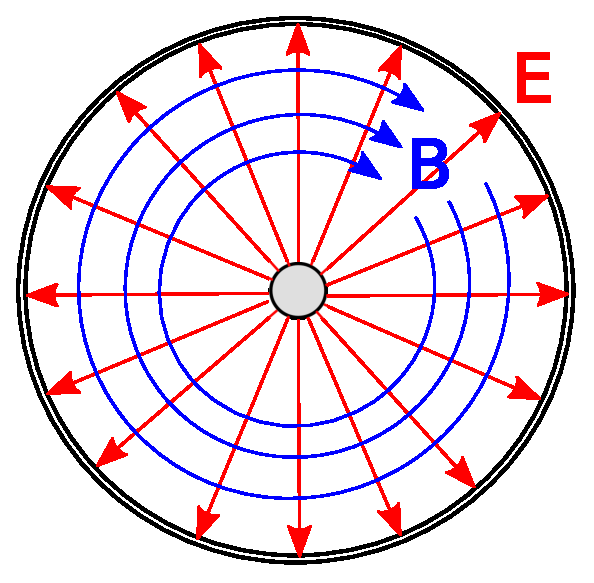
\includegraphics[width=1.5in]{modules/m0143_fCoaxFieldStructure.eps}
}}{A cross-sectional view of a coaxial transmission line. The inner conductor is represented by a gray-filled circle.  The electric field, "E", is represented by red arrows pointing outward from the inner conductor to the outer conductor which is represented by a larger concentric circle. The magnetic field, "B", is represented by concentric, circular blue arrows between the insulating jacket and the inner conductor. The arrows indicate a clockwise direction.}
\end{center} 
\caption{\label{m0143_fCoaxFieldStructure}Structure of the electric and magnetic fields within coaxial line.  In this case, the wave is propagating away from the viewer.}
\end{figure}
 
Expressions for the equivalent circuit parameters $C'$ and $L'$ for coaxial lines can be obtained from basic electromagnetic theory.
It is shown in Section~\ref{m0113_Capacitance_of_Coaxial_Line} that the capacitance per unit length is
%
\begin{equation}
C' = \frac{2\pi\epsilon_s}{\ln\left(b/a\right)}
\label{m0143_eCp}
\end{equation}
%
where $a$ and $b$ are the radii of the inner and outer conductors, respectively.
Using analysis shown in Section~\ref{m0125_Inductance_of_a_Coaxial_Transmission_Line}, the inductance per unit length is
%
\begin{equation}
L' = \frac{\mu_0}{2\pi}\ln\left(\frac{b}{a}\right)
\label{m0143_eLp}
\end{equation}
%
The loss conductance $G'$ depends on the conductance $\sigma_s$ of the spacer material, and is given by 
%
\begin{equation}
G' = \frac{2\pi\sigma_s}{\ln\left(b/a\right)}
\end{equation}
%
This expression is derived in Section~\ref{m0105_Conductance_DC}.

The resistance per unit length, $R'$, is relatively difficult to quantify.
One obstacle is that the inner and outer conductors typically consist of different materials or compositions of materials.
The inner conductor is not necessarily a single homogeneous material; instead, the inner conductor may consist of a variety of materials selected by trading-off between conductivity, strength, weight, and cost.
Similarly, the outer conductor is not necessarily homogeneous; for a variety of reasons, the outer conductor may instead be a metal mesh, a braid, or a composite of materials.
Another complicating factor is that the resistance of the conductor varies significantly with frequency, whereas $C'$, $L'$, and $G'$ exhibit relatively little variation from their electro- and magnetostatic values.
These factors make it difficult to devise a single expression for $R'$ that is both as simple as those shown above for the other parameters and generally applicable.
Fortunately, it turns out that the low-loss 
\index{transmission line!low loss}
conditions $R'\ll\omega L'$ and $G'\ll\omega C'$ are often applicable,\footnote{See Section~\ref{m0083_Lossless_Transmission_Lines} for a reminder about this concept.} so that $R'$ and $G'$ are important only if it is necessary to compute loss. 

Since the low-loss conditions are often met, a convenient expression for the characteristic impedance 
\index{characteristic impedance!coaxial cable}
is obtained from Equations~\ref{m0143_eCp} and \ref{m0143_eLp} for $L'$ and $C'$ respectively:
%
\begin{flalign}
Z_0 & \approx \sqrt{\frac{L'}{C'}} ~~~\mbox{(low-loss)} \nonumber \\
    & = \frac{1}{2\pi}\sqrt{\frac{\mu_0}{\epsilon_s}}\ln{\frac{b}{a}} 
\end{flalign}
%
The spacer permittivity can be expressed as $\epsilon_s=\epsilon_r\epsilon_0$ where $\epsilon_r$ is the relative permittivity of the spacer material.
Since $\sqrt{\mu_0/\epsilon_0}$ is a constant, the above expression is commonly written
%
\begin{equation}
Z_0 \approx \frac{60~\Omega}{\sqrt{\epsilon_r}} \ln{\frac{b}{a}} ~~~\mbox{(low-loss)}
\end{equation}
%
Thus, it is possible to express $Z_0$ directly in terms of parameters describing the geometry ($a$ and $b$) and material ($\epsilon_r$) used in the line, without the need to first compute the values of components in the lumped-element equivalent circuit model.

Similarly, the low-loss approximation makes it possible to express the phase velocity $\nu_p$ directly in terms the spacer permittivity:
\index{phase velocity!coaxial cable}
%
\begin{flalign}
\nu_p & \approx \frac{1}{\sqrt{L'C'}} ~~~\mbox{(low-loss)} \nonumber \\
      & = \frac{c}{\sqrt{\epsilon_r}}
\end{flalign}
%
since $c\triangleq 1/\sqrt{\mu_0\epsilon_0}$.
In other words, the phase velocity in a low-loss coaxial line is approximately equal to the speed of electromagnetic propagation in free space, divided by the square root of the relative permittivity of the spacer material. 
Therefore, the phase velocity in an air-filled coaxial line is approximately equal to speed of propagation in free space, but is reduced in a coaxial line using a dielectric spacer.

%ORB EXAMPLE
~\\ \begin{example} 
\begin{mdframed}[backgroundcolor=brown!20,linecolor=brown!20]\raggedright 
RG-59 
\index{RG-59}
Coaxial Cable. 
\\~\\
RG-59 is a very common type of coaxial line.
Figure~\ref{m0143_fRG-59} shows a section of RG-59 cut away so as to reveal its structure.
The radii are $a\cong 0.292$~mm and $b\approx 1.855$~mm (mean), yielding $L'\approx 370$~nH/m.
The spacer material is polyethylene having $\epsilon_r\cong 2.25$, yielding $C'\approx 67.7$~pF/m.
The conductivity of polyethylene is $\sigma_s\cong 5.9 \times 10^{-5}$~S/m, yielding $G'\approx 200~\mu$S/m.
Typical resistance per unit length $R'$ is on the order of $0.1~\Omega$/m near DC, increasing approximately in proportion to the square root of frequency. 

From the above values, we find that RG-59 satisfies the low-loss criteria 
$R'\ll\omega L'$ for $f\gg 43$~kHz and 
$G'\ll\omega C'$ for $f\gg 470$~kHz.
Under these conditions, we find $Z_0 \approx \sqrt{L'/C'} \cong 74~\Omega$.    
Thus, the ratio of the potential to the current in a wave traveling in a single direction on RG-59 is about $74~\Omega$.

The phase velocity of RG-59 is found to be $v_p \approx 1/\sqrt{L'C'} \cong 2 \times 10^8$~m/s, which is about 67\% of $c$.  In other words, a signal that takes 1~ns to traverse a distance $l$ in free space requires about 1.5~ns to traverse a length-$l$ section of RG-59. 
Since $v_p = \lambda f$, a wavelength in RG-59 is 67\% of a wavelength in free space.

Using the expression 
%
\begin{equation}
\gamma = \sqrt{\left(R'+j\omega L'\right)\left(G'+j\omega C'\right)}
\end{equation} 
%
with $R'=0.1~\Omega$/m, and then taking the real part to obtain $\alpha$, we find $\alpha\sim 0.01$~m$^{-1}$.  So, for example, the magnitude of the potential or current is decreased by about 50\% by traveling a distance of about 70~m. 
In other words, $e^{-\alpha l} = 0.5$ for $l \sim 70$~m at relatively low frequencies, and increases with increasing frequency.    

\end{mdframed} 

\begin{figure}
\begin{center}
\pdftooltip{{  % note double braces
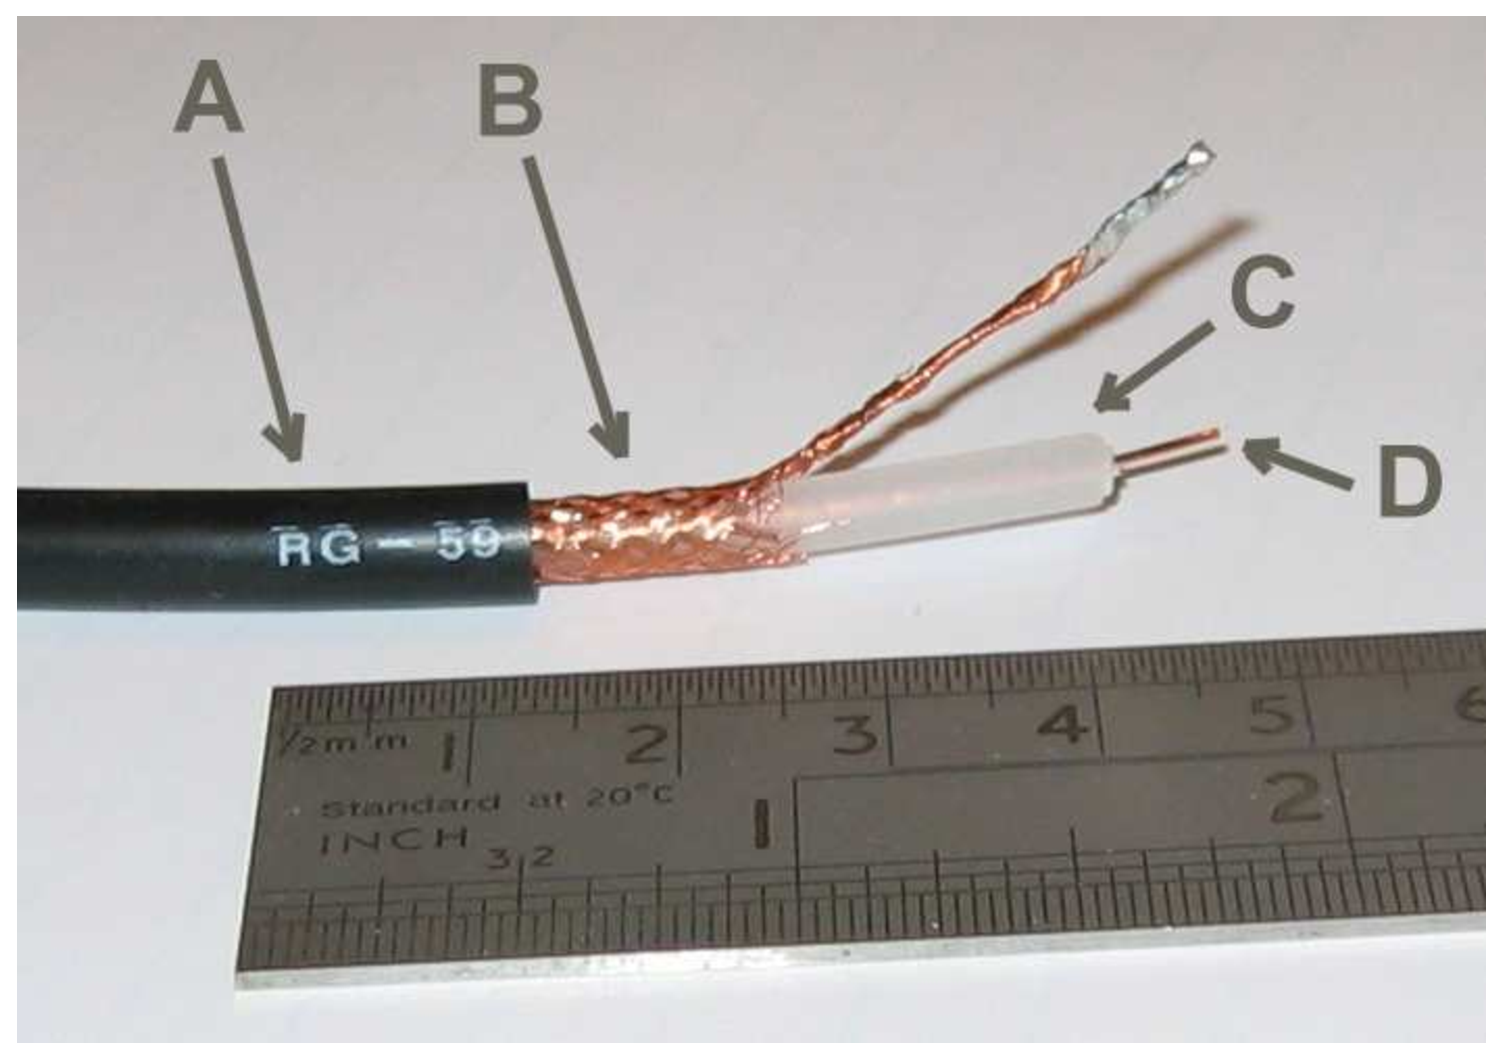
\includegraphics[width=2.5in]{modules/m0143_fRG-59.eps}
% https://en.wikipedia.org/wiki/File:RG-59.jpg
}}{A photo of a dissected coaxial line. A ruler is sitting next to the coaxial line for reference. About 3 cm of the line is missing the insulating jacket. The braided outer conductor is removed over a 1.5 cm section of the dielectric spacer. A 0.5 cm section of dielectric spacer is removed, exposing the inner conductor.}
\end{center} 
\centerline{\scriptsize 
\copyright~\hyperref[m0143_fRG-59_Credit]{Arj} 
\href{https://creativecommons.org/licenses/by-sa/3.0/}{CC BY~SA 3.0} 
} 
\caption{
\label{m0143_fRG-59}
RG-59 coaxial line. A: Insulating jacket. B: Braided outer conductor. C: Dielectric spacer. D: Inner conductor. 
}
\end{figure}

\end{example}

%%%%%%%%%%%%%%%%%%%%%%%%%%%%%%%%

{\bf Additional Reading:}
\begin{itemize}
\item ``\href{https://en.wikipedia.org/wiki/Coaxial_cable}{Coaxial cable}'' on Wikipedia. \emph{Includes descriptions and design parameters for a variety of commonly-encountered coaxial cables.}
\item ``\href{https://en.wikipedia.org/wiki/Single-ended_signaling}{Single-ended signaling}'' on Wikipedia.
\item Sec.~8.7 (``Differential Circuits'') in S.W.~Ellingson, \emph{Radio Systems Engineering}, Cambridge Univ.\ Press, 2016. 
\end{itemize}

\index{transmission line!coaxial|)}
